\subsection{Toward a common standard}\label{sec:terminology}

%\ugh{\textbf{ICSE 10-years} good example of traceability for specific purpose without generalization !}
%

%\nb{1}{The incoherency problem.} 
The ubiquitous presence of traceability in software literature spreading through out different fields and application scenarios has hampered the use of a consistent and shared terminology around the key traceability concepts\footnote{A trace-based paper was awarded the most influential paper in the past 10 years at one of the main venue on software engineering (ICSE)~\cite{ko2008-whyline-debugging}. The work introduced a novel trace-based approach to debugging that prominent industrials made use of with brio. Yet, if debugging has made a buzz, traceability remained a secondary concern. (Even though "trace" is mention 46 times in the 10 pages paper).}.  
In this perspective, we argue that the "incoherency problem" arises in traceability research~\cite{watts2017-incoherency-problem}. Even if an individual article made a claim that withstood rigorous testing and statistical analysis, it might not use the same words as an adjacent article, or it would use the same words but intend different meanings~\cite{bouillon2013-survey-on-usage-scenario-requirements-traceability-in-practice,antoniol2017-traceability-grand-challenges}. %\jc{kind of a bold claim, can you back it up?} 
For instance, the term \textit{traceability} is used to designate both the ability to trace system elements, and the traceability links (the relations) themselves. Regarded as a mere mandatory constraint in safety critical domains or as a lucky by-product of model transformation execution in automated model manipulation, no \textit{de-facto} or \textit{de-juro} standard rules the landscape of traceability investigations~\cite{mader2009-motivation-matters-in-traceability-practitioner-survey}.


In this section, we first review the different usages of traceability in the literature and then we integrate them in a single metamodel and set of term definitions that we believe will help to understand and compare the different traceability proposals we will be analyzing later on. 

% and in industrial scenarios as those depicted above through many a research field has hampered a clear and constructive terminology to emerge. %Vast unstructured use of traceability, without standard, leads to a lack in communication (when "collaboration and traceability management have the potential to be mutually beneficial")~\cite{wohlrab2020-traceability-organization-process-culture}. 
%In this perspective, we argue that the "incoherency problem" arises in traceability research. Even if an individual article made a claim that withstood rigorous testing and statistical analysis, it might not use the same words as an adjacent article, or it would use the same words but intend different meanings~\cite{watts2017-incoherency-problem}.


\subsubsection{Different interpretations of the traceability concept}
Traceability research was born with a definition coined by Gotel \textit{et al.}: "Requirements  traceability  refers  to  the  ability  to  describe and  follow  the life of a requirement, in both a forwards  and backwards direction", a broad definition focused on the ability to link requirements to code or design elements of a system~\cite{gotel1994}. Decades later, traceability still refers mainly to \textit{requirement-driven approaches} that aim at understanding the semantics of requirements~\cite{bouillon2013-survey-on-usage-scenario-requirements-traceability-in-practice,badreddin2014-req-traceability-model-based-approach}. %\jc{Is there any reference that supports this claim? Is this something that you saw when analyzing the survey papers?} 
While approaches vary in their means and goals, the attention remains primarily focused on the dependencies linking specifications to design and code artefacts.

Similarly, \textit{modeling approaches} see traceability techniques as useful tools aimed at linking artefacts at different levels of abstraction (and different phases and increment of the software life cycle)~\cite{mader2007-tracing-unified-process,tekinerdogan2007-metamodel-for-tracing-concers-accross-life-cycle}, and \textit{transformation approaches} make profit of the use of automated transformations to generate (and maintain) automatically trace artefacts~\cite{galvao2007-survey-traceability-in-MDE}. Others use \textit{feature traceability} to refer to the ability to locate features in software artefacts~\cite{meinicke2017-feature-traceability}.

%The number of survey exploded around the year 2010 (see \Fig{fig:publicationyears-trace}) and numerous studies were published the following years. 
In all cases, we notice a division of knowledge into four main areas: i) strategizing traceability, ii) the creation, maintenance and evolution of trace artefacts, iii) the identification and record of trace links, and iv) the usability of trace representations~\cite{winkler2010-survey-traceability-and-MDE,antoniol2017-traceability-grand-challenges}). The first is higher level concern, the three others are first order features of tracing ability.

\begin{itemize}
	\item \textbf{Strategizing traceability} means defining an explicit purpose to a traceability approach including the means to achieve it and a way to measure the (remaining) distance to that goal. 
	\item \textbf{Trace artefact management} means the definition of trace artefact representations, their characteristics, design, and variability. The emphasis is here put on the language definition with metamodels and frameworks, the typing of the links, and the maintenance of the coherence in traceability artefacts. In this area, model artefacts and traces co-evolution is an important concern in the model-driven paradigm.
	\item \textbf{Trace link identification} designates the identification of traces in a software system, be it a post-requirement assisted elicitation, or a live record during a system execution. Most of the literature in this area focus on the automation of the identification process by means of machine learning techniques.
	\item \textbf{Trace usability} means ways to make use of existing traces. This includes the tool support for automated task on existing trace artefacts such as the persistence, retrieval and analysis.
\end{itemize}



\subsubsection{Key traceability terms' definitions}
We propose some general definitions for the most frequently encountered terms while searching for and studying solutions for traceability in any of the above categories. These definitions aim to encompass and unify all the different uses and vision of traceability depicted above. 

Note that these definitions (same for the metamodel following up in the next subsection) do not aim to cover all the different visions on traceability but provide a common core generic enough to be then adapted to specific scenarios. This is why we do this work before conducting the survey as this is a preliminary step, based on our knowledge of the field, to help us classify the survey results and not a result of the survey itself.

%\jc{Maybe clarify that these definitions aim to encompass and unify all the different uses and vision of traceability depicted above}.

\begin{itemize}
	\renewcommand\labelitemi{--}
	\item[--] \textbf{Traceability} is the ability to trace different artefacts of a system (of systems). It is defined in the IEEE Standard Glossary of Software Engineering Terminology \cite{ieeeglossary-se} as 
	\begin{enumerate}
		\item The degree to which a relationship can be established between two or more products of the development process, especially products having a predecessor–successor or master–subordinate relationship to one another. [...]
		\item The degree to which each element in a software development product establishes its reason for existing.
	\end{enumerate}
	
	
	\item A \textbf{trace} is a path from one artefact to another. Composed of atomic \textbf{links} that directly relate artefacts with each others. The representation of traces, their data structure and behaviour, is defined in a \textbf{traceability information model} (TIM), or traceability metamodel~\cite{drivalos2009-engineering-DSL-for-traceability}. In both cases it defines at the language level the concepts and relationships available for tracing. With the manifolds of traceability purposes, no common representation has emerged yet. 
	
	\item A \textbf{trustee} is the human actor responsible for an artefact.
	
	\item A \textbf{link} is a relationship between two artefacts. The \textbf{type of the relationship} informs about its semantics. Typing is a primary concern in conceptual modeling in general~\cite{olive2002-representation-of-generic-relationship-types-in-modeling}. The heterogeneous nature of traceability applications, and the importance of links in that domain confers relation types a peculiar attention since it helps understand the rationale behind relationship - it informs not only \textit{how} artefacts are linked but also \textit{why}~\cite{mader2009-motivation-matters-in-traceability-practitioner-survey}. It is to note that most of the work aiming at modeling "traceability" actually models traceability links. This suites the OMG standard definition of traceability which consider the only input/output of transformations~\cite{winkler2010-survey-traceability-and-MDE}. 
	
	\item An \textbf{artefact} can be any element of a system - \eg unstructured documentation, code, design diagrams, test cases and suites... The nature of artefacts follows two main dimensions: the development process they belong to (\eg specification, design, implementation, test), and their type (\eg unstructured natural language, grammar-based code, model-based artefact). The \textbf{granularity of artefacts} is the level to which artefacts can be decomposed into sub parts. We call a \textbf{fragment}, the resulting product of the decomposition of an artefact. A fragment can be itself broken down into smaller parts (or sub-fragments), and so forth and so on. For example, a software requirement document could include a guideline for certification which in turn could include sub-sections and a model-level definition of their implications.
	
	\item \textbf{Trace integrity} is the degree of reliability that bares a trace. It is a measure that includes both the age of a trace, the volatility of artefacts targeted by the trace, and the automation level of tracing features. This indication is supported by \textbf{evidences} that can be quantitative or qualitative. For example, how long (how many versions ago) has the trace been identified in the system? Or, is has the trace been identified manually or automatically? Is there an automated co-evolution mechanism between traces and targeted artefacts? What is the level of experience of the trustee who identified it? 
	The volatility of source and target artefacts are also factors that may influence the relevance and accuracy of a trace.
	
	\item \textbf{Pre-requirement and post-requirement} traceability refer to, respectively, traces identified during the edification of specifications and during the implementation (design and code) step of a specification~\cite{gotel1994}.
	The IEEE Guide for Software Requirements Specifications mentions \textbf{forward} and \textbf{backward} traceability, referring to the ability to follow traceability links from a source to a specific artefact, or the opposite from the artefact to its source, respectively~\cite{ieeeglossary-req} but, technically, the direction of traceability link (from source to target, or from target to source) does not make a difference.
	
	\item \textbf{Explicit links} refer to artefacts that explicitly link to each other in the concrete syntax. \textbf{Implicit links} show artefacts bondage at a syntactic or semantic level without explicit link (\textit{e.g.,} binary class and source code artefact with the same name - or the same prefix - are "linked" to each others)~\cite{paige2010-MDE-Traceability-classifications}.
	
	\item \textbf{Vertical traceability} refers to the linkage between artefacts at different levels of abstraction (\textit{e.g.,} derives, implements, inherits) whereas \textbf{horizontal traceability} refers to artefacts at the same level (\textit{e.g.,} uses, depends on). 
	
	\item \textbf{Time related traceability} goes along two dimensions (\textit{e.g.,} the evolution of (a group of) elements through successive development tasks or the evolution of artefact properties during an execution of the system.) \cite{yu2012-maintainging-invariant-traceability}.
\end{itemize}



\subsubsection{Traceability metamodel}
\begin{figure}[h]
	\centering
	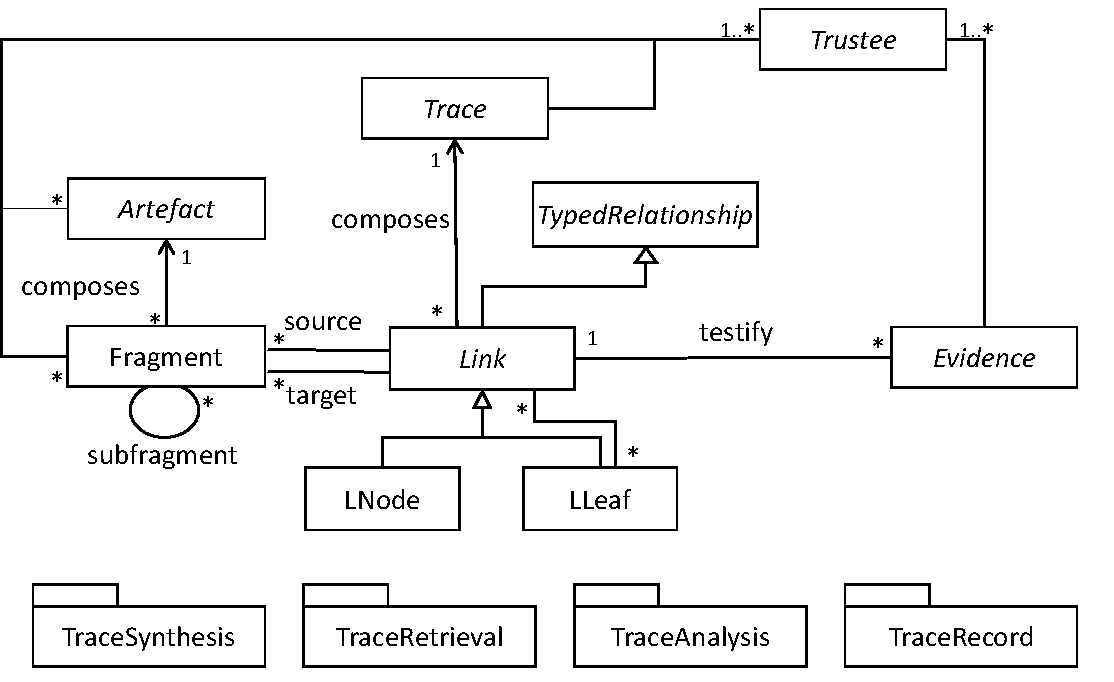
\includegraphics[width=.6\linewidth]{images/metamodel}
	\caption{Indicative metamodel.}
	\label{fig:metamodel}
\end{figure}

As a first contribution of this work, we propose a generic traceability metamodel that helps to formalize better the relationships between the terms described above. This metamodel will also be used through out the paper to discuss and compare traceability approaches, together with the feature model presented later on. At its core, the metamodel comprises a generic representation of tracing artefacts: the links composing a trace, their respective evidences and trustees, and the decomposition of trace and system elements. As pictured in \Fig{fig:metamodel}, a \texttt{trace} is composed of a set of arborescent \texttt{links}. Taken in its broader sense, a trace is a forest of links that connects one or more source \texttt{fragment} to one or more target fragment. Links are \texttt{typed relationships}. This typing allow for a semantic definition specific to the targeted application domain. %For example, a code generator will connect configuration files with the executable of the generator, themselves connected to the generated source code. There is not necessarily a need for all links to be represented but it might be of great help to have a structure robust enough to decide which ones of these links must be represented for analysis. 
Each link is associated with an \texttt{evidence} that testifies the level of confidence of that link. The reliability is affected whether the link has been created manually or inferred automatically, if there is a rule that assess if the link is still valid or not, if it is not deprecated, and so forth and so on. A link refers to fragments of artefacts. These fragments are decomposition of artefacts that can be decomposed as well. Since traceability is strongly advised for validation and certification of safety intensive software systems, the relation between software or trace artefact and their (human) \texttt{trustee} must also be considered explicitly.



